\documentclass{beamer}
%\documentclass[aspectratio=169]{beamer}
\usepackage{ctex, hyperref}
\usepackage[T1]{fontenc}

% other packages
\usepackage{latexsym,amsmath,xcolor,multicol,booktabs,calligra}
\usepackage{graphicx,pstricks,listings,stackengine}
\usepackage{animate}
\usepackage{algorithm, algorithmic}
\usepackage{ulem}
\usepackage{tcolorbox}
\tcbuselibrary{skins}


\author[XJTU数学建模课程汇报]{计算机2205\hspace{0.1cm}李雨轩\\
计算机2204\hspace{0.1cm}马润东\\
计算机2203\hspace{0.1cm}易兰昕\\
计算机2203\hspace{0.1cm}赵文文}
\title{Lamprey与元胞自动机}
\subtitle{XJTU数学建模课程汇报}
\date{2024 年 4 月 2 日}
\institute{Team. 26}
\usepackage{RenminUniv}


\begin{document}
\kaishu
\begin{frame}
    \titlepage

    \begin{figure}[htpb]
        \begin{center}
            
\includegraphics[width=0.3\linewidth]{pic/title.png}
        \end{center}
    \end{figure}
\end{frame}

\begin{frame}
\tableofcontents[sectionstyle=show,subsectionstyle=show/shaded/hide,subsubsectionstyle=show/shaded/hide]
\end{frame}



\section{元胞自动机}

\begin{frame}{元胞自动机:介绍}
    
    \begin{block}{元胞自动机 (Cellular Automaton)}
        元胞自动机是一种离散的、分布式的计算模型,由一系列相同结构的元胞组成,每个元胞在离散的时间和空间上演化,根据一组规则进行状态的转换。
    \end{block}
    
    \begin{itemize}
        \item \textbf{元胞 (Cell)}:空间中的单个单元,通常组成一个规则的网格。
        \item \textbf{状态 (State)}:每个元胞可以处于有限的状态之一。
        \item \textbf{邻居 (Neighborhood)}:每个元胞有一组相邻元胞,通常定义为固定范围内的相邻元胞。
        \item \textbf{转换规则 (Transition Rule)}:定义了根据元胞的当前状态和邻居的状态来确定下一个时刻元胞的状态的规则。
    \end{itemize}

\end{frame}

\begin{frame}{元胞自动机:形式化定义}
    
    \begin{block}{形式化定义}
        元胞自动机由一个五元组 $({\displaystyle {\mathcal {L}}}, {\displaystyle {\mathcal {E}}}_1, {\displaystyle {\mathcal {E}}}_2, {\displaystyle {\mathcal {N}}}, {\displaystyle {\mathcal {R}}})$ 完全定义了其行为。
        
        \[
            {\displaystyle {\mathcal {CA}}}_{modified} \overset{def}{=} ({\displaystyle {\mathcal {L}}}, {\displaystyle {\mathcal {E}}}_1, {\displaystyle {\mathcal {E}}}_2, {\displaystyle {\mathcal {N}}}, {\displaystyle {\mathcal {R}}})
        \]
    \end{block}
    
   \begin{itemize}
        \item ${\displaystyle {\mathcal {L}}}$ 是一个二维网格,用于表示细胞的空间布局。${\displaystyle {\mathcal {E}}}_1$ 和 ${\displaystyle {\mathcal {E}}}_2$ 表示一组有限状态,每个细胞在任何时刻都处于 ${\displaystyle {\mathcal {E}}}_1 \times {\displaystyle {\mathcal {E}}}_2 $ 中。
        \item ${\displaystyle {\mathcal {N}}}$ 是邻域定义,它确定了哪些相邻细胞的状态会影响当前细胞状态的更新。
        \item ${\displaystyle {\mathcal {R}}}: ({\displaystyle {\mathcal {E}}}_1 \times {\displaystyle {\mathcal {E}}}_2 )^{\left|{\displaystyle {\mathcal {N}}}\right|} \rightarrow {\displaystyle {\mathcal {E}}}_1 \times {\displaystyle {\mathcal {E}}}_2 $ 是转换函数,它根据细胞的当前状态及其邻居确定细胞的下一个状态。这里 $\left|{\displaystyle {\mathcal {N}}}\right|$ 是邻域 ${\displaystyle {\mathcal {N}}}$ 中的细胞数量。
\end{itemize}
    
\end{frame}


\begin{frame}{元胞自动机与模拟}
    \hspace{2em} 元胞自动机 (Cellular Automata , CA) 具有强大的空间运算能力 , 常用于自组织系统演变过程的研究 。 它是一种时间 、 空间 、 状态都离散 , 空间相互作用和时间因果关系都为局部的网格动力学模型 , 具有模拟复杂系统时空演化过程的能力 。 它这种 “自下而上” 的研究思路 , 充分体现了复杂系统局部的个体行为产生全局、有秩序模式的理念 。 

\end{frame}


\begin{frame}{元胞自动机的历史}
    \hspace{2em} 细胞自动机最早由美籍数学家冯·诺依曼(John von Neumann)在1950年代为模拟生物细胞的自我复制而提出,但是并未受到学术界重视。直到1970年,英国数学家约翰·何顿·康威(John Horton Conway)设计了生命游戏并经马丁·葛登在《科学美国人》杂志上介绍,才吸引了科学家们的注意。此后,英国学者史蒂芬·沃尔夫勒姆(Stephen Wolfram)对初等元胞机256种规则所产生的模型进行了深入研究,并用熵来描述其演化行为,将细胞自动机分为平稳型、周期型、混沌型和复杂型。
\end{frame}

\begin{frame}{一些概念上的解释}

\begin{block}{元胞空间}
    形状、大小
\end{block}

\begin{block}{元胞邻居}
    定义域
\end{block}

\begin{block}{元胞规则}
    转移方程
\end{block}

\begin{block}{元胞边界}
    有限/无限
\end{block}
\end{frame}


\section{题目重述}
\begin{frame}{题目重述}

大多数动物物种存在雌雄两性,但有些会呈现性别比例偏差,称为适应性性别比变异。例如,Lamprey的性别比受到食物可用性的影响,导致雌性或雄性比例的变化。

\begin{block}{任务}
    关注性别比及其依赖于局部条件的问题,特别是对于Lamprey。
    \begin{itemize}
        \item 当Lamprey的种群可以改变其性别比时,对更大的生态系统有什么影响?
        \item 对Lamprey的种群有什么优点和缺点?
        \item 在Lamprey的性别比发生变化的情况下,生态系统的稳定性有什么影响?
        \item 具有可变性别比的Lamprey种群的生态系统能否为生态系统中的其他物种,如寄生虫,提供优势?
    \end{itemize}
\end{block}

\end{frame}

\begin{frame}{可行方案与困境}
\begin{block}{常规思路}
\begin{itemize}
    \item Lotka-Volterra 捕食者-猎物模型:
        基于两个微分方程,描述了捕食者和猎物种群的变化随时间的动态过程。
    \item 生态位模型:
        通常使用特征向量来表示物种在多维资源空间中的位置,从而探讨物种之间的竞争和共存关系。
    \item 地理信息系统 (GIS) 模型:
        使用地理信息系统技术,结合地理数据和生态学数据,进行空间分析和模拟
    \item 马尔科夫链模型:
        用于描述物种在时间上的变化和转移。马尔科夫链模型可以用于研究种群的迁徙、种群的状态转换、物种在不同生境中的分布等问题。
\end{itemize}
\end{block}

\begin{block}{面临的问题}
    存在的问题:数据不好找、参数不好确定...
\end{block}

\end{frame}


\section{基于元胞自动机的模拟}

\subsection{生命游戏}

\begin{frame}{生命游戏}
\begin{block}{规则}
    \begin{itemize}
        \item 如果一个细胞周围有三个细胞为生,则该细胞为生(即该细胞原先为死则转为生)
        \item 如果细胞周围有两个细胞为生,则该细胞不变
        \item 在其他情况下,该细胞为死
    \end{itemize}
\end{block}
    \begin{columns}[T]
    \begin{column}{0.5\textwidth}
        \begin{figure}[htpb]
            \centering
            \animategraphics[height=1.0in,autoplay,loop]{30}{./gif/Game_of_life_animated_LWSS-}{0}{27}
            \caption{生命游戏}
        \end{figure}
    \end{column}
    \begin{column}{0.5\textwidth}
        \begin{figure}[htpb]
            \centering
            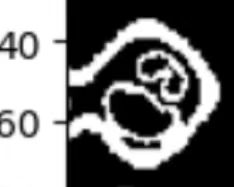
\includegraphics[height=1.0in]{./pic/mm.jpg}
            \caption{\sout{人像}}
        \end{figure}
    \end{column}
\end{columns}
\end{frame}


\begin{frame}{生命游戏举例}
\begin{minipage}[t]{0.45\textwidth}
生命游戏中的较复杂演化模式:“播种机”模式不断生成“高斯帕机枪”来制造“滑翔机”
\end{minipage}%
\hfill
\begin{minipage}[t]{0.45\textwidth}
生命游戏中的一种可持续繁殖模式:“高斯帕机枪”不断制造“滑翔机”
\end{minipage}

\vspace{1em}

\begin{minipage}[t]{0.45\textwidth}
\centering
\animategraphics[height=1.0in,autoplay,loop]{30}{./gif/Conways_game_of_life_breeder_animation-}{459}{498}
\end{minipage}%
\hfill
\begin{minipage}[t]{0.45\textwidth}
\centering
\animategraphics[height=1.0in,autoplay,loop]{30}{./gif/Gospers_glider_gun-}{1}{29}
\end{minipage}

\end{frame}


\subsection{生态系统模拟}


\begin{frame}{元胞自动机与生态模拟的关联}
以下是元胞自动机可以用来模拟生态环境的几个原因:
\begin{itemize}
    \item 局部互动性: 元胞自动机中的每个单元格只与其周围的邻居单元格交互,这种局部互动反映了自然界中生物个体之间的相互作用。生态系统中的物种往往与其周围环境和其他物种进行交互。
    \item 简单规则的复杂性: 元胞自动机的规则通常非常简单,但是当大量的单元格按照这些规则交互时,可以产生出复杂的全局行为。这种复杂性反映了生态系统中群体行为的出现。
    \item 适应性和演化: 元胞自动机中的规则可以随着时间演化和变化,从而模拟生态系统中物种的适应性和演化过程。通过调整规则,可以模拟出不同环境条件下生物的适应性和生态系统的稳定性。
\end{itemize}

\end{frame}


\begin{frame}{元胞自动机模拟的缺陷}
\begin{block}{尽管元胞自动机模拟生态环境有一定优势,但也存在缺陷}
    \begin{itemize}
    \item 简化的模型: 元胞自动机模型是对现实的简化和抽象,可能忽略了许多真实世界中复杂的因素和相互作用。
    \item 参数选择困难: 定义模拟中的状态和规则需要合适的参数选择,这可能是一个困难的过程。参数的选择可能会影响模拟结果的准确性和可靠性。
    \item 计算资源消耗: 当模拟规模较大时,元胞自动机模型可能需要大量的计算资源和时间来完成模拟。这可能限制了模拟的规模和复杂性。
\end{itemize}
\end{block}

于是就有学者提出用一系列 CA 来模拟生态系统不同方面的特性 。 为更好地认识和了解 CA , 可以将复杂的生态系统进行分解 , 用不同的 CA 模拟生态系统的不同特征 。

\end{frame}


\begin{frame}{生命游戏启示下的一个新思路}
\hspace{2em} Lamprey是可以改变性别比例的生物,性别取决于幼鱼阶段的生长速度。
关于这一主题的研究对我们理解不同性别比例物种的影响做出了重大贡献。
利用元胞自动机模型模拟不同性别比例的Lamprey,探究能够改变性别比例的Lamprey的优缺点,以及不同性别比例对生态系统的影响,并定量评估Lamprey性别比例对生态系统的影响。

\hspace*{\fill}

\hspace{2em}我们不必严格拘泥于收集到的数据,通过比较模型模拟的不同规则下的结果,使分析和解决问题变得更加容易和方便。
\end{frame}

\begin{frame}{生态系统模拟方法}
\begin{block}{难点在于规则}
    \begin{itemize}
        \item 在生态系统中添加合适的规则:…
        \item 稳定值试出来作为初值...
        \item 找趋于稳定值的规则...
    \end{itemize}    
\end{block}
\begin{block}{实现起来并不复杂}
    \begin{tcolorbox}[colback=white,colframe=black!50!white]
    \begin{algorithmic}
        \FOR{each cell in the grid}
            \STATE Calculate the number of live neighbors surrounding the cell
            \STATE Update 
        \ENDFOR
        \STATE Update the grid with the new cell states
    \end{algorithmic}
    \end{tcolorbox}
    
\end{block}

\end{frame}

\begin{frame}{模拟结果}
    \begin{figure}[htpb]
        \centering
        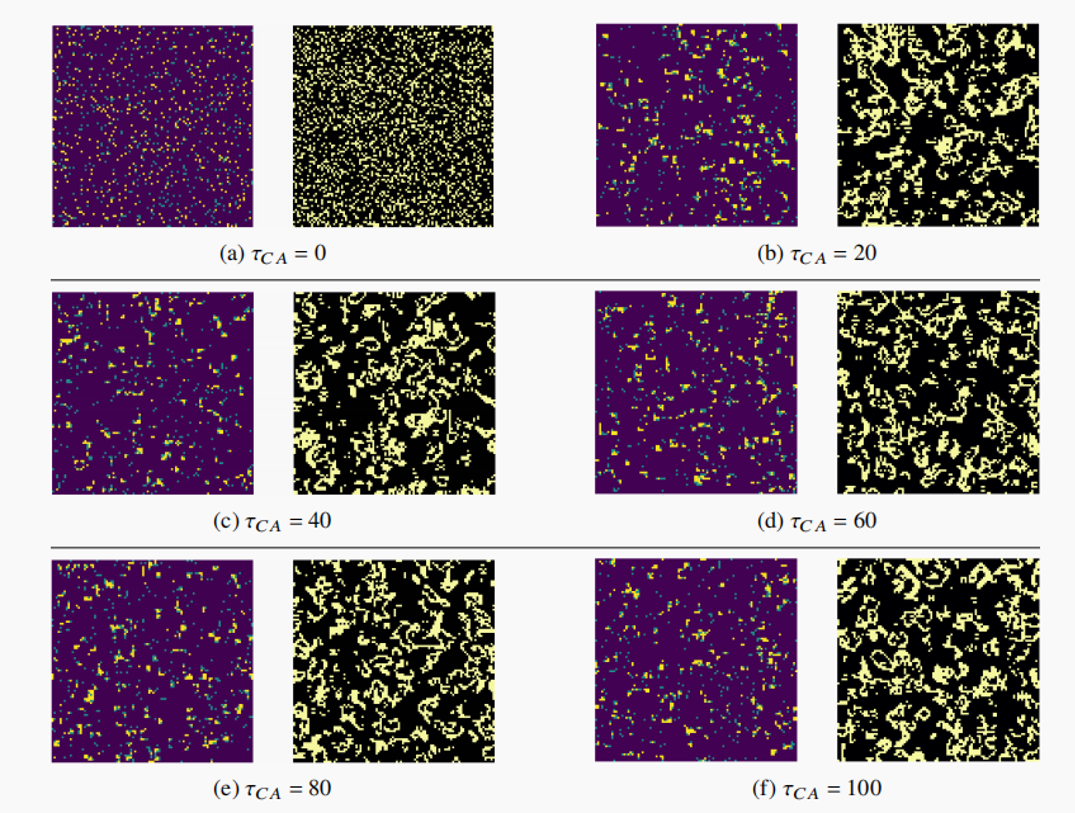
\includegraphics[width=0.6\linewidth]{./pic/stimulate.png}
        \caption{stimulate}
    \end{figure}
\end{frame}







\subsection{原建模问题分析}

\begin{frame}{问题2}
    \hspace{2em} 我们在环境性别决定模拟模型中添加“灾难”,得到了对“灾难”的两种生态系统响应。利用随时间变化的猎物和Lamprey数量的数据,我们分析了Lamprey的优点和缺点:优点:改变性别比例有助于维持不同环境条件下Lamprey种群的稳定性和恢复力。缺点:当Lamprey处于极度食物短缺的情况下,种群的遗传多样性和长期生存能力可能面临风险。
\end{frame}

\begin{frame}{问题3}
    \hspace{2em} 我们在问题2中添加一个新的生态系统(有猎物的生态系统,以及性别比例始终为1:1的Lamprey的生态系统),并获取发生灾害的三个生态系统的数据。基于AHP‑Topsis模型,构建了生态系统稳定性评估模型,确定Lamprey对生态系统稳定性的影响。最终,三个生态系统稳定性得分分别为44.98、21.89和33.13。因此,能够调节性别比例的Lamprey对生态系统的稳定性具有显着影响,并显着促进其稳定性。
\end{frame}

\begin{frame}{问题4}
    \hspace{2em} 我们向问题1的生态系统添加新物种——寄生虫。我们模拟在环境性别决定模拟模型的帮助下,这个新的生态系统并比较了两个系统中寄生虫的数量,从而得出结论Lamprey的性别比例可能导致寄生虫数量增加。
\end{frame}


\section{稳定性评估模型}

\begin{frame}{生态系统稳定性的四个决定性要素}
\begin{block}{层次分析法(AHP)}
    \begin{itemize}
        \item 物种数量的波动性
        \item 周期的长度
        \item 生态系统的抵抗力
        \item 生态系统的恢复力
    \end{itemize}
\end{block}

利用层次分析法(AHP),我们可以得出上述四项的权重因数
    \begin{figure}[htpb]
        \centering
        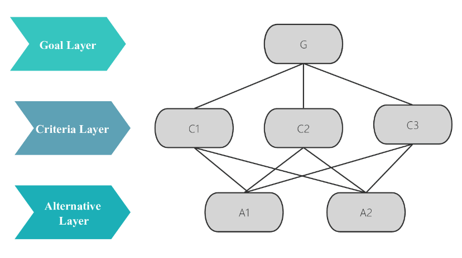
\includegraphics[width=0.6\linewidth]{./pic/Layout.png}
        \caption{层次模型}
    \end{figure}

\end{frame}


\begin{frame}{构建层次模型}
    \begin{itemize}
        \item 目标层:评估生态系统的稳定性
        \item 准则层:
            \begin{itemize}
                \item 物种种群变异性:指生态系统中物种数量的波动。
                \item 种群变化周期:生态系统中自然周期的持续时间。             
                \item 生态系统复原力:生态系统从干扰中恢复到扰动前的状态的能力。
                \item 生态系统抵抗力:生态系统在结构和功能发生不重大变化的情况下承受干扰的能力。
            \end{itemize}
            
        \item 方案层
            \begin{itemize}
                \item 系统$A$:猎物和可以改变性别的Lamprey种群。
                \item 系统$B$:猎物和不能改变性别的Lamprey种群。             
                \item 系统$C$:猎物和性别比例始终为1:1的Lamprey种群。
            \end{itemize}
    \end{itemize}

\end{frame}


\begin{frame}{构造判断矩阵与一致性检验}
    \begin{itemize}
        \item 构造判断矩阵:判断矩阵 $A$ 中的每个元素 $a_{ij}$ 表示因素 $i$ 相对于因素 $j$ 的重要性,其中 $a_{ij} = 1/a_{ji}$。
        \item 一致性检验:计算矩阵 $A$ 的最大特征根 $\lambda$,然后计算一致性指标 $CI$,其中 $CI = (\lambda_{max} - n)/(n - 1)$。一致性指标越接近0,一致性越好,我们引入随机一致性指标 $RI$ 来衡量 $CI$ 的大小,$RI = (\sum_{i=0}^{n} CI_i) / n$。显然,$RI$ 的大小与判断矩阵的阶数有关,因此我们引入检验系数 $CR$,$CR = CI / RI$。当 $CR < 0.1$ 时,认为该判断矩阵通过一致性检验。
        \item 计算标准权重:对比较矩阵进行归一化,求得如下的权重向量。$\boldsymbol{\omega} = (\omega_1, \omega_2, \dots, \omega_n)$,其中 $\omega_i = \left(\prod_{j=1}^{n} a_{ij}\right)^{\frac{1}{n}} / \left(\sum_{k=1}^{n} \left(\prod_{j=1}^{n} a_{kj}\right)^{\frac{1}{n}}\right), (i=1,2,\dots,n)$。
    \end{itemize}
\end{frame}


\begin{frame}{计算生态系统稳定性得分}
\begin{itemize}
    \item 我们按照模型一模拟生态系统$A$,系统$B$,系统$C$,假设在$t_0$ 时间之前,系统处于稳定状态,猎物和Lamprey的数量处于周期性变化的稳定状态。在$t_0$时间,发生灾难,导致猎物数量急剧减少,持续$m$年后猎物和Lamprey的数量恢复稳定
    \item 综合考虑物种数量的波动性、周期的长度、生态系统的抵抗力、生态系统的恢复力,再对结果进行归一化处理我们获得描述生态系统稳定性的矩阵
    $\mathbf{M} = \begin{bmatrix}
        m_{11} & \cdots & m_{1n} \\
        \vdots & \ddots & \vdots \\
        m_{n1} & \cdots & m_{nn}
    \end{bmatrix}$。

\end{itemize}
    

\end{frame}


\section{结论}
\begin{frame}{结论}
\begin{itemize}
    \item 当Lamprey种群能改变性别比例时,猎物数量减少,Lamprey数量增加。
    \item 优势:改变性别比例有助于增加Lamprey种群在不同环境条件下的稳定性和恢复力。
    \item 劣势:当Lamprey种群处于极度食物短缺的情况下,雌性Lamprey的数量会急剧减少,性别比例失衡 ,影响遗传多样性和种群的长期生存能力。
    \item 能够调节性别比例的Lamprey种群对生态系统的稳定性具有重大影响, 大大提高其稳定性。 
    \item Lamprey性别比例的变化可能导致寄生虫数量增加。
    
\end{itemize}

\end{frame}



\begin{frame}
\begin{center}
	{\Huge\calligra Thanks!}
\end{center}
\hspace*{\fill}
\hspace*{\fill}
\hspace*{\fill}
\hspace*{\fill}
\hspace*{\fill}
\hspace*{\fill}
\hspace*{\fill}
\hspace*{\fill}
\hspace*{\fill}
\hspace*{\fill}
{\small\calligra made by Li Yuxuan}
\end{frame}


\end{document}